\documentclass[10pt,a4paper]{article}
\usepackage[margin=16mm,headsep=5mm,footskip=8mm]{geometry}
\usepackage{amsmath,amssymb,booktabs,array,tabularx,multicol,graphicx,xcolor,enumitem,fancyhdr,hyperref,float}
\usepackage[most]{tcolorbox}
\definecolor{navy}{HTML}{17324D}\definecolor{blue}{HTML}{2D6A8A}\definecolor{pale}{HTML}{EEF5F8}\definecolor{warn}{HTML}{8A4B08}\definecolor{green}{HTML}{2E6B4F}
\hypersetup{colorlinks=true,linkcolor=blue,urlcolor=blue}
\setlist{nosep,leftmargin=*}\setlength{\parindent}{0pt}\setlength{\parskip}{4pt}
\newcommand{\dd}{\,\mathrm{d}}\newcommand{\unit}[1]{\,\mathrm{#1}}
\newtcolorbox{quick}[1][]{colback=pale,colframe=blue,boxrule=.6pt,arc=1mm,title=#1,fonttitle=\bfseries}
\newtcolorbox{trap}[1][]{colback=yellow!8,colframe=warn,boxrule=.6pt,arc=1mm,title=#1,fonttitle=\bfseries}
\newtcolorbox{example}[1][]{colback=green!5,colframe=green,boxrule=.6pt,arc=1mm,title=#1,fonttitle=\bfseries}
\pagestyle{fancy}\fancyhf{}\lhead{ENME601 Thermodynamics}\rhead{Half-Semester Resource v2}\cfoot{\thepage}
\begin{document}
\begin{titlepage}\centering\vspace*{23mm}
{\Huge\bfseries Thermodynamics\\Half-Semester Resource v2\par}\vspace{5mm}
{\Large ENME601 --- Weeks 1--6\par}\vspace{11mm}
{\large Expanded open-book reference with explanations, modelling decisions, derivations, worked examples, table workflows, device templates and exam checks.\par}
\vfill
\begin{quick}[Purpose]
This version deliberately contains more explanation than v1. Use it to decide what model applies and why; use the separate Tutorial Booklet v2 for all 61 rewritten tutorial questions and expanded solutions. Numerical pure-substance values should always be checked against the current \textit{Property Tables 2026}.
\end{quick}
\vfill 20 August 2026
\end{titlepage}
\tableofcontents\newpage

\section{How to turn a word problem into a thermodynamic model}
Thermodynamics problems become manageable when the physical model is decided before the arithmetic. The same numerical data can lead to different equations depending on whether mass crosses the boundary, whether the process is steady, and whether the substance is a gas, liquid, or two-phase mixture.

\subsection{The seven-line exam setup}
Write these lines before substituting numbers:
\begin{enumerate}
\item \textbf{System:} name the matter or region being studied.
\item \textbf{Boundary:} state whether mass can cross it; draw heat and work arrows.
\item \textbf{Knowns and unknowns:} include units and state numbers.
\item \textbf{Assumptions:} justify each simplification physically.
\item \textbf{Properties:} identify the phase and source of $u,h,v,s,c_p,c_v$.
\item \textbf{Balances:} write the full mass and energy equations.
\item \textbf{Checks:} sign, units, magnitude, phase limits and conservation.
\end{enumerate}

\begin{quick}[Problem-type selector]
\begin{tabularx}{\textwidth}{>{\bfseries}p{.20\textwidth}X X}
\toprule Cue & Model & First equation\\\midrule
Sealed tank, piston-cylinder, fixed mass & closed system & $Q-W=\Delta U+\Delta KE+\Delta PE$\\
Pipe, nozzle, turbine, compressor, valve & control volume & mass balance, then SFEE\\
Water/R-134a with $P,T,x,v,u,h$ & pure substance & classify phase, then choose table\\
Gas far from saturation & ideal gas & $PV=mRT$ plus energy relation\\
Solid or liquid heating & incompressible & $\Delta u\simeq c\Delta T$\\
Engine, refrigerator, heat pump & cyclic device & energy relation plus efficiency or COP\\\bottomrule
\end{tabularx}
\end{quick}

\subsection{Sign convention and units}
This resource uses heat into the system as positive and work done by the system as positive:
\[
Q-W=\Delta E.
\]
Expansion boundary work is normally positive; compression work is negative. If a question asks for ``work required,'' report the positive magnitude of the work input and label it clearly.

Useful identities:
\[
1\unit{kPa\,m^3}=1\unit{kJ},\qquad 1\unit{kW}=1\unit{kJ/s},\qquad T[\unit K]=T[^{\circ}\unit C]+273.15.
\]
A velocity term $V^2/2$ is J/kg in SI, so divide by 1000 before adding it to an enthalpy in kJ/kg.

\begin{trap}[Simplification is not assumption]
Do not write ``$\Delta KE=0$'' as an assumption without a reason. Write ``inlet and outlet speeds are small compared with the enthalpy scale, so $\Delta KE$ is neglected.'' A crossed-out term must correspond to a physical statement.
\end{trap}

\section{Week 1 --- systems, state, properties and pressure}
\subsection{Systems and boundaries}
A \textbf{closed system} contains a fixed mass. Its boundary may move, so heat and work can cross even though mass cannot. An \textbf{open system}, or control volume, is a selected region through which mass may flow. An \textbf{isolated system} exchanges neither mass nor energy.

Examples:
\begin{itemize}
\item Sealed rigid tank: closed system, fixed boundary, no boundary work.
\item Piston-cylinder: closed system, moving boundary, possible boundary work.
\item Turbine casing: open control volume, mass and energy cross.
\item Thermos flask idealisation: approximately isolated over a short interval.
\end{itemize}

\subsection{Properties, state and equilibrium}
Extensive properties scale with system size: $m,V,U,H,E$. Intensive properties do not: $P,T,\rho,v$. A specific property is an extensive property divided by mass.
\[
\rho=\frac{m}{V},\qquad v=\frac{V}{m}=\frac1\rho,
\qquad \gamma=\rho g.
\]
For a simple compressible pure substance, two independent intensive properties determine the state. Independence matters: inside the saturation dome, $P$ and $T$ are linked by the saturation relation, so another property such as quality or specific volume is required.

Thermodynamic equilibrium includes thermal, mechanical, phase and chemical equilibrium. A quasi-equilibrium process passes through states close enough to equilibrium that properties and a path such as $P(V)$ remain meaningful.

\subsection{Processes, cycles and path functions}
Isothermal means constant $T$; isobaric constant $P$; isochoric constant $V$; adiabatic $Q=0$. A cycle returns all state properties to their starting values, so $\Delta U_{cycle}=0$, although the net heat and work need not be zero.

Heat and work are path functions: they describe energy crossing the boundary during a process. Internal energy, enthalpy, pressure and temperature are properties of a state.

\subsection{Absolute, gauge and vacuum pressure}
\[
P_{abs}=P_{atm}+P_{gauge},\qquad P_{abs}=P_{atm}-P_{vac}.
\]
Use absolute pressure in ideal-gas equations and property tables. Gauge pressure may be negative, but absolute pressure cannot.

For a static fluid,
\[
\frac{\dd P}{\dd z}=-\rho g,\qquad \Delta P=\rho g\Delta h
\]
when density is approximately constant. Move downward through a fluid and pressure increases; move upward and it decreases. At a common elevation in the same connected static fluid, pressure is the same.

\begin{example}[Room-air properties]
A room has $V=300\unit{m^3}$ and contains $350\unit{kg}$ of air:
\[
\rho=350/300=1.167\unit{kg/m^3},\quad v=0.857\unit{m^3/kg},\quad \gamma=\rho g=11.44\unit{N/m^3}.
\]
The calculation describes a fixed quantity of air, so the chosen system is closed even if the real room has small leakage.
\end{example}

\begin{trap}[Week 1 traps]
Steady does not mean spatially uniform. Temperature difference in $^\circ$C equals the difference in K, but temperature ratios require K. Specific weight is weight per volume, not mass per volume.
\end{trap}

\section{Week 2 --- energy, heat, work and ideal gases}
\subsection{Forms of stored energy}
\[
E=U+KE+PE,
\qquad e=u+\frac{V^2}{2}+gz.
\]
For a finite mass,
\[
\Delta KE=\frac{m(V_2^2-V_1^2)}{2},\qquad \Delta PE=mg(z_2-z_1).
\]
Internal energy is microscopic molecular energy. Kinetic and potential energies describe the system as a whole.

\subsection{Heat and work interactions}
Heat transfer is energy crossing a boundary solely because of a temperature difference. Work is any other organised energy transfer. Common modes include:
\[
\dot W_{shaft}=\tau\omega=2\pi N\tau,
\quad W_{spring}=\tfrac12k(x_2^2-x_1^2),
\quad W_{lift}=mg\Delta z.
\]
Electrical work can be written $W_{elec}=VI\Delta t$ for constant voltage and current.

For a closed system,
\[
Q-W=\Delta U+\Delta KE+\Delta PE.
\]
For a stationary closed system this reduces to $Q-W=\Delta U$, not automatically to $Q=\Delta U$: all work modes must first be considered.

\subsection{Power versus energy}
Energy is an amount, measured in kJ. Power is a rate, measured in kW. Reaching the same speed in less time requires the same ideal kinetic-energy change but a greater average power.
\[
\dot W_{avg}=\frac{W}{\Delta t}.
\]

\subsection{Ideal-gas model}
An ideal gas obeys
\[
Pv=RT,\qquad PV=mRT,\qquad R=\frac{R_u}{M}.
\]
For a fixed mass between two equilibrium states,
\[
\frac{P_1V_1}{T_1}=\frac{P_2V_2}{T_2}.
\]
Use absolute pressure and kelvin. The ideal-gas model is often good at low density and far from the saturation region; it is poor for liquids and near-condensation vapours.

For an ideal gas, internal energy and enthalpy depend primarily on temperature:
\[
\Delta u=\int c_v(T)\dd T,\qquad \Delta h=\int c_p(T)\dd T,
\qquad c_p-c_v=R.
\]

\begin{example}[Energy and power]
If an ideal lossless car reaches the same final speed in $5\unit s$ or $3.5\unit s$, $\Delta KE$ is unchanged. The power ratio is
\[
\frac{\dot W_{3.5}}{\dot W_5}=\frac{5}{3.5}=1.429.
\]
The faster acceleration needs about 43\% greater average power.
\end{example}

\begin{trap}[Do not overuse $mc\Delta T$]
$Q=mc\Delta T$ is not a universal law. $mc\Delta T$ estimates a property change under a suitable model; the first law must still account for work, kinetic/potential changes and phase change.
\end{trap}

\section{Week 3 --- pure substances and property tables}
\subsection{Phase behaviour}
\begin{figure}[H]\centering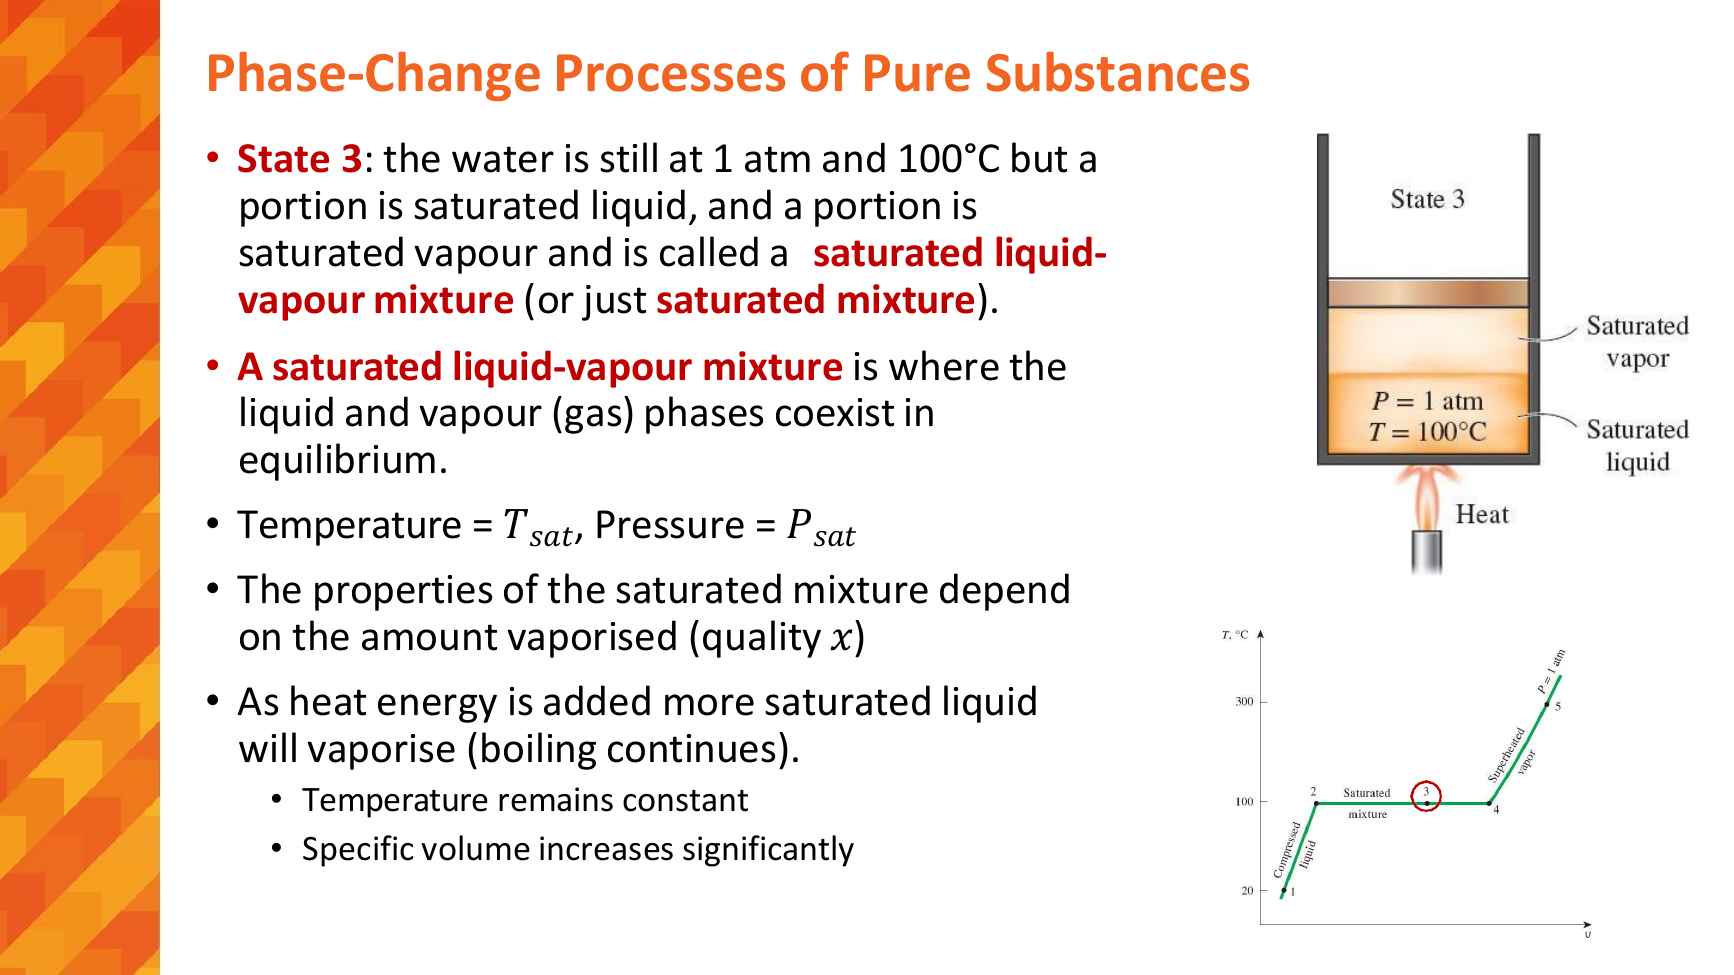
\includegraphics[width=.82\textwidth]{figures/week3-phase.png}\caption*{Pure-substance phase regions and the saturation dome.}\end{figure}
A pure substance may be compressed liquid, saturated mixture, saturated vapour or superheated vapour. At saturation, phase change occurs at linked $P_{sat}$ and $T_{sat}$.

At a known pressure:
\begin{center}
\begin{tabular}{lll}\toprule
Comparison & Region & Table\\\midrule
$T<T_{sat}(P)$ & compressed/subcooled liquid & compressed-liquid table or approximation\\
$T=T_{sat}(P)$ & saturated state & quality or another property needed\\
$T>T_{sat}(P)$ & superheated vapour & superheated table\\\bottomrule
\end{tabular}
\end{center}
At a known temperature, make the equivalent comparison using pressure.

\subsection{Quality and mixture properties}
Quality is the vapour mass fraction:
\[
x=\frac{m_g}{m_f+m_g},\qquad 0\le x\le1.
\]
For $y\in\{v,u,h,s\}$,
\[
y=y_f+xy_{fg},\qquad y_{fg}=y_g-y_f,
\qquad x=\frac{y-y_f}{y_{fg}}.
\]
Quality is undefined for compressed liquid and superheated vapour.

\subsection{Enthalpy and why it appears}
\[
h=u+Pv.
\]
The $Pv$ term represents the flow work required to push a stream across a control-volume boundary. Combining it with internal energy makes open-system equations much cleaner.

\subsection{Interpolation}
For a property $y$ between rows $X_1$ and $X_2$,
\[
y=y_1+\frac{X-X_1}{X_2-X_1}(y_2-y_1).
\]
Write the two bracketing rows before calculating. Never interpolate between different phase regions or different property tables.

\begin{example}[Interpolated saturation pressure]
At $222.5^\circ$C, bracket between $220^\circ$C with $2319.6\unit{kPa}$ and $225^\circ$C with $2549.7\unit{kPa}$:
\[
P=2319.6+\frac{222.5-220}{225-220}(2549.7-2319.6)=2434.65\unit{kPa}.
\]
\end{example}

\subsection{Compressed-liquid approximation}
When a compressed-liquid table is unavailable,
\[
y(T,P)\approx y_f(T),
\]
particularly for $v$ and $u$. A pressure-corrected enthalpy estimate is
\[
h(T,P)\approx h_f(T)+v_f(T)[P-P_{sat}(T)].
\]
State that this is an approximation.

\begin{quick}[Property-table decision tree]
Substance $\rightarrow$ two independent intensive properties $\rightarrow$ saturation comparison $\rightarrow$ region $\rightarrow$ correct table $\rightarrow$ interpolation $\rightarrow$ sanity check. A two-phase property must lie between its $f$ and $g$ values.
\end{quick}

\section{Week 4 --- closed-system energy analysis}
\begin{figure}[H]\centering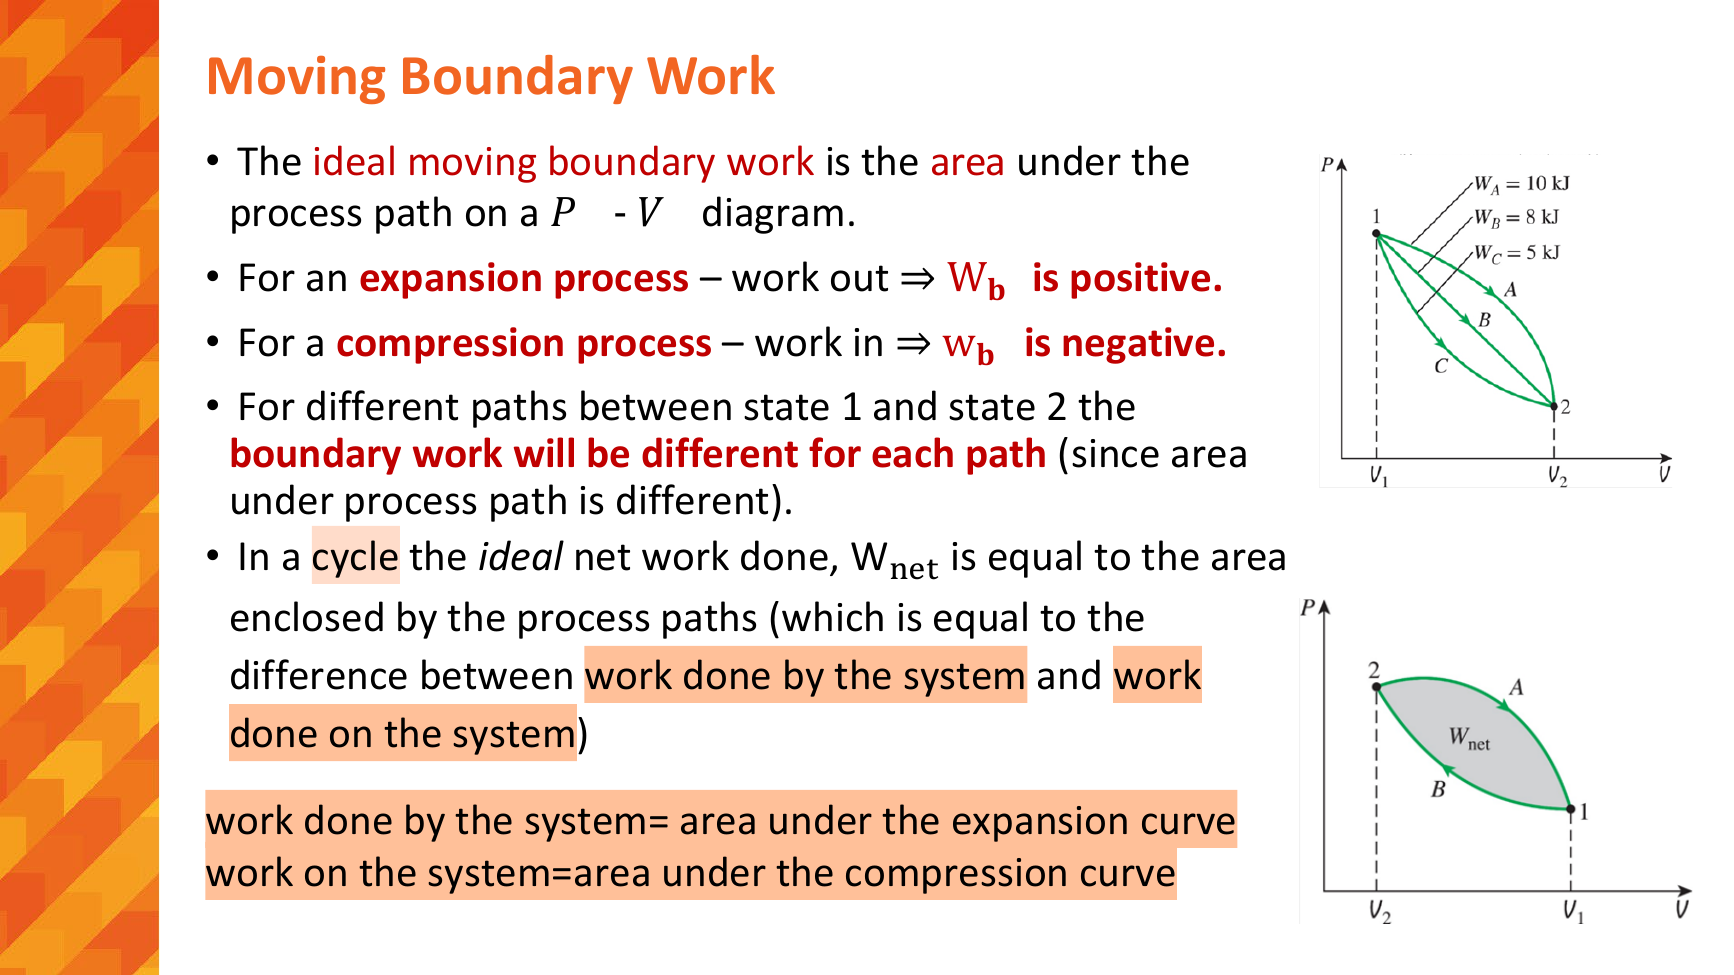
\includegraphics[width=.82\textwidth]{figures/week4-pv.png}\caption*{Boundary work as area beneath a quasi-equilibrium $P$--$V$ path.}\end{figure}
\subsection{Boundary work}
For a quasi-equilibrium moving boundary,
\[
W_b=\int_{V_1}^{V_2}P\dd V.
\]
The path matters. Two processes with the same endpoints can produce different work because the area under their $P$--$V$ curves differs.

\begin{center}
\begin{tabular}{ll}\toprule Process model & Work\\\midrule
Constant pressure & $P(V_2-V_1)$\\
Rigid tank & $0$\\
Isothermal ideal gas & $mRT\ln(V_2/V_1)$\\
Polytropic $PV^n=C$, $n\ne1$ & $(P_2V_2-P_1V_1)/(1-n)$\\
Linear spring path & $(P_1+P_2)(V_2-V_1)/2$\\\bottomrule
\end{tabular}
\end{center}
A reversible adiabatic ideal gas follows $PV^k=C$. Adiabatic alone is insufficient; reversibility/quasi-equilibrium is also required.

\subsection{Combining work with the first law}
\[
Q-W=\Delta U+\Delta KE+\Delta PE.
\]
For a stationary rigid tank with only heat transfer, $Q=m(u_2-u_1)$. For a constant-pressure piston-cylinder with boundary work as the only work,
\[
Q=m(h_2-h_1).
\]
This enthalpy result follows from combining $\Delta U$ with $P\Delta V$; it is not a different conservation law.

\subsection{Specific heats and model selection}
For ideal gases,
\[
\Delta u\approx c_{v,avg}\Delta T,
\qquad \Delta h\approx c_{p,avg}\Delta T.
\]
Use $c_v$ with internal energy and $c_p$ with enthalpy. For incompressible substances,
\[
\Delta u\approx c\Delta T,
\qquad \Delta h\approx c\Delta T+v\Delta P.
\]

\begin{example}[Linear compression path]
If $P=aV+b$, $a=-1500\unit{kPa/m^3}$, $b=400\unit{kPa}$, and $V$ decreases from $0.2$ to $0.1\unit{m^3}$,
\[
W_b=\frac a2(V_2^2-V_1^2)+b(V_2-V_1)=-17.5\unit{kJ}.
\]
The negative sign is expected because work is done on the gas.
\end{example}

\begin{trap}[Week 4 traps]
Constant pressure does not mean constant temperature. Isothermal does not mean constant pressure unless a two-phase saturation relation enforces it. A rigid tank has $W_b=0$ but may still exchange heat or other work.
\end{trap}

\section{Week 5 --- control volumes and steady-flow devices}
\begin{figure}[H]\centering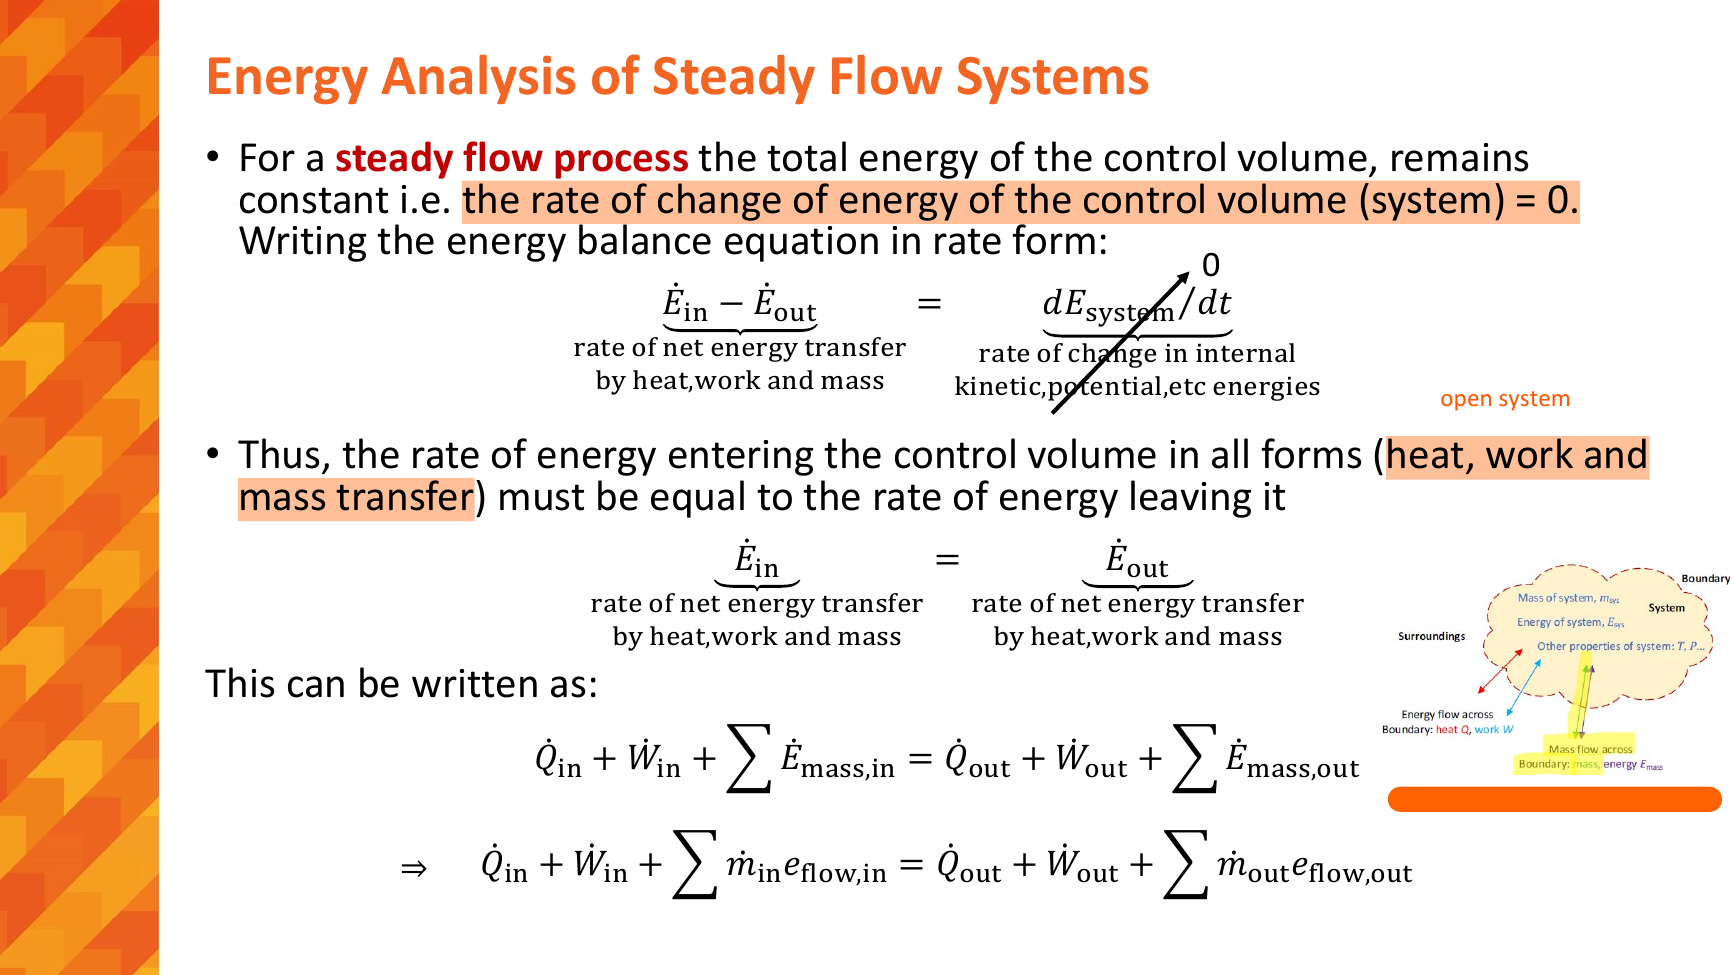
\includegraphics[width=.82\textwidth]{figures/week5-control-volume.png}\caption*{A control volume with mass and energy crossing its boundary.}\end{figure}
\subsection{Mass balance}
The general mass balance is
\[
\frac{dm_{CV}}{dt}=\sum\dot m_{in}-\sum\dot m_{out}.
\]
At steady state, accumulation is zero. For one-dimensional flow,
\[
\dot V=V_{avg}A,
\qquad \dot m=\rho\dot V=\rho V_{avg}A=\frac{\dot V}{v}.
\]
A filling tank is transient because its contained mass changes, even if the inlet flow itself is constant.

\subsection{Steady-flow energy equation}
A flowing stream carries
\[
h+\frac{V^2}{2}+gz.
\]
With $Q$ into and shaft work out positive,
\[
\dot Q-\dot W=\sum_{out}\dot m\left(h+\frac{V^2}{2}+gz\right)-\sum_{in}\dot m\left(h+\frac{V^2}{2}+gz\right).
\]
For one inlet and outlet,
\[
\dot Q-\dot W=\dot m\left[(h_2-h_1)+\frac{V_2^2-V_1^2}{2}+g(z_2-z_1)\right].
\]

\subsection{Device templates}
\begin{tabularx}{\textwidth}{>{\bfseries}p{.18\textwidth}X X}
\toprule Device & Common justified assumptions & Reduced relation\\\midrule
Nozzle/diffuser & steady, adiabatic, no shaft work, negligible $\Delta PE$ & $h_1+V_1^2/2=h_2+V_2^2/2$\\
Turbine & adiabatic, negligible $\Delta KE,\Delta PE$ & $\dot W_{out}=\dot m(h_1-h_2)$\\
Compressor & adiabatic, negligible $\Delta KE,\Delta PE$ & $\dot W_{in}=\dot m(h_2-h_1)$\\
Pump & incompressible liquid, small temperature rise & $w_{in}\simeq v(P_2-P_1)$\\
Throttle & adiabatic, no shaft work, negligible $\Delta KE,\Delta PE$ & $h_1=h_2$\\
Mixing chamber & steady, adiabatic, no work & $\sum\dot m h_{in}=\sum\dot m h_{out}$\\
Heat exchanger & whole device externally adiabatic, no work & hot-stream loss = cold-stream gain\\\bottomrule
\end{tabularx}

\begin{example}[Adiabatic compressor]
For air compressed from $293.15$ to $573.15\unit K$, table values $h_1=293.32$ and $h_2=578.88\unit{kJ/kg}$ give
\[
w_{in}=h_2-h_1=285.56\unit{kJ/kg}.
\]
If $\dot m=0.01426\unit{kg/s}$, then $\dot W_{in}=4.08\unit{kW}$.
\end{example}

\begin{example}[Throttling valve]
R-134a entering as saturated liquid at $700\unit{kPa}$ is throttled to $160\unit{kPa}$. The usual throttle assumptions give $h_2=h_1$. The exit is found at the lower pressure with this enthalpy; it may be a mixture even though the inlet was liquid. Throttling is not generally isothermal or isentropic.
\end{example}

\section{Week 6 --- second law, engines and refrigeration}
\begin{figure}[H]\centering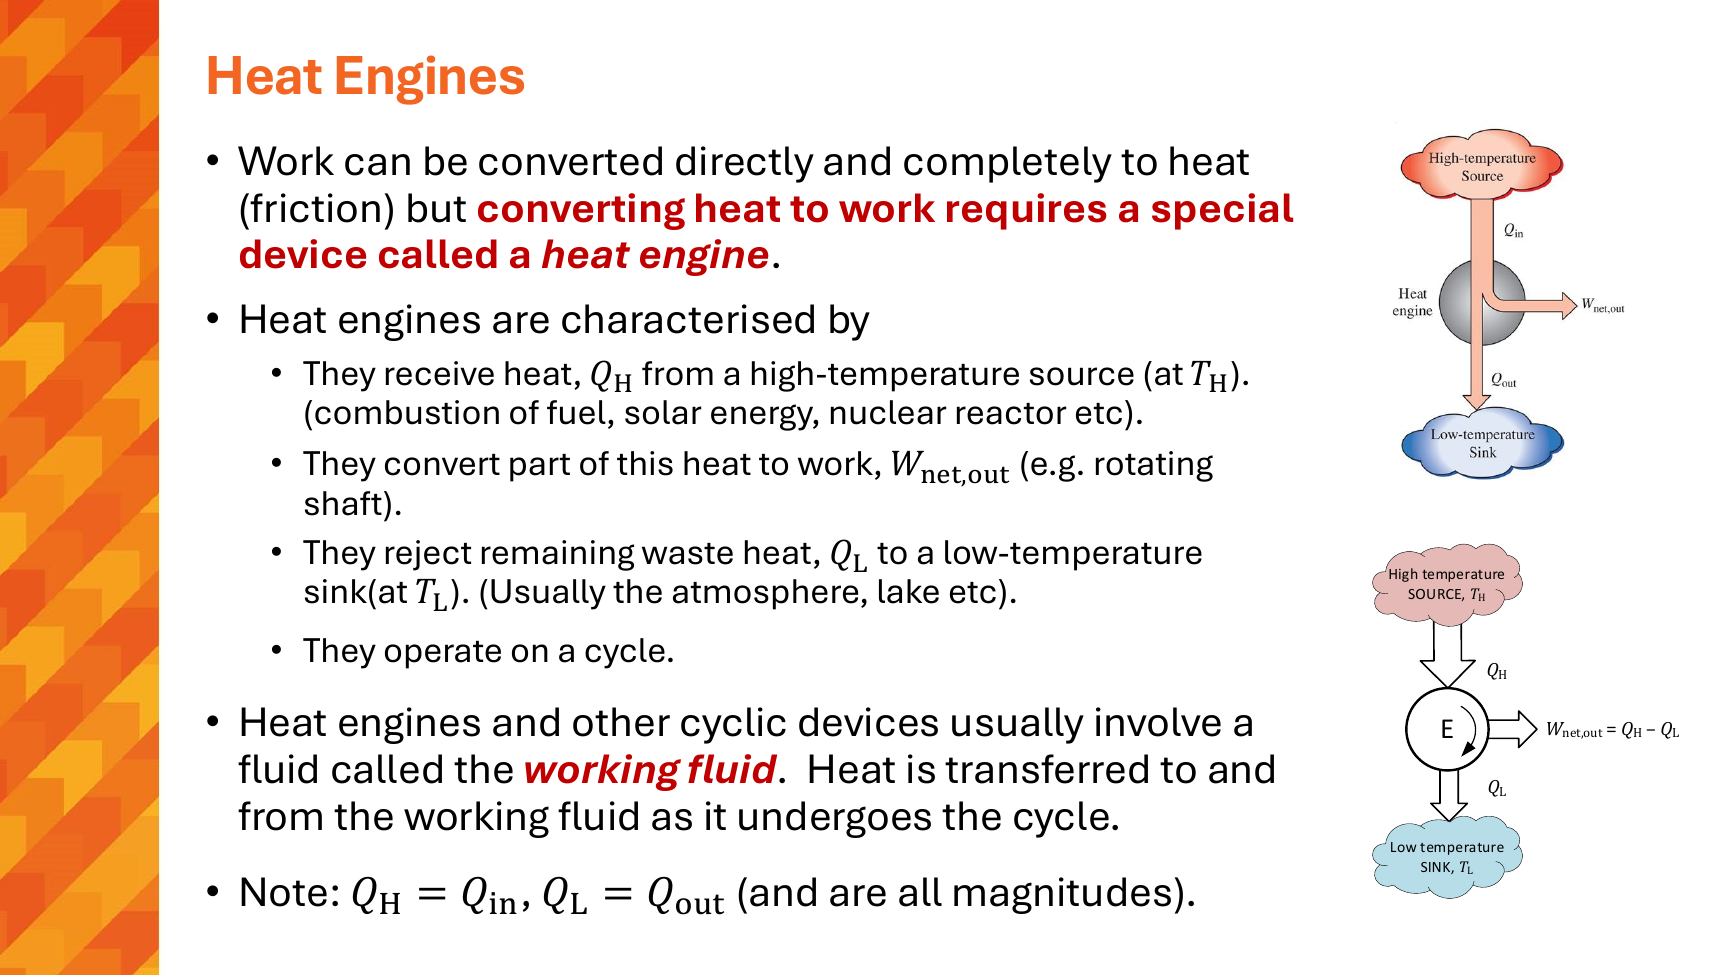
\includegraphics[width=.82\textwidth]{figures/week6-engine.png}\caption*{Heat-engine energy flows between hot and cold reservoirs.}\end{figure}
\subsection{Why the second law is needed}
The first law constrains energy quantity but not direction or attainable performance. The second law explains why heat flows naturally from hot to cold, why cyclic heat engines must reject heat, and why real processes lose work potential.

Kelvin--Planck: no cyclic heat engine can convert all heat from a single reservoir into work. Clausius: heat cannot flow from cold to hot without an external effect such as work input.

\subsection{Heat engines}
\[
W_{net,out}=Q_H-Q_L,
\qquad \eta_{th}=\frac{W_{net,out}}{Q_H}=1-\frac{Q_L}{Q_H}.
\]
Efficiency must lie between zero and one.

\subsection{Refrigerators and heat pumps}
\[
W_{net,in}=Q_H-Q_L,
\]
\[
COP_R=\frac{Q_L}{W_{net,in}},
\qquad COP_{HP}=\frac{Q_H}{W_{net,in}}=COP_R+1.
\]
COP can exceed one because the desired heat transfer includes energy moved from the other reservoir; COP is not an efficiency.

\subsection{Carnot limits}
For reversible operation between reservoirs at absolute temperatures $T_H$ and $T_L$,
\[
\eta_{rev}=1-\frac{T_L}{T_H},
\]
\[
COP_{R,rev}=\frac{T_L}{T_H-T_L},
\qquad COP_{HP,rev}=\frac{T_H}{T_H-T_L}.
\]
No real device operating between the same reservoirs can exceed these limits.

\subsection{Irreversibilities}
Sources include friction, turbulence, unrestrained expansion, mixing, combustion, electrical resistance and heat transfer across a finite temperature difference. Reversible devices are ideals that give maximum turbine work, minimum compressor work and limiting COP/efficiency.

\begin{example}[Plant efficiency]
A plant produces $150\unit{MW}$ while coal supplies $500\unit{MW}$ of thermal energy:
\[
\eta=150/500=0.30=30\%.
\]
The rejected energy rate is approximately $350\unit{MW}$ if other stored-energy changes are negligible.
\end{example}

\begin{example}[Heat-pump COP]
For $COP_{HP}=2.5$, each $1\unit{kWh}$ of work can deliver $2.5\unit{kWh}$ to the house because $1.5\unit{kWh}$ is absorbed from outside:
\[
Q_H=Q_L+W_{in}=1.5+1.0=2.5\unit{kWh}.
\]
No first-law violation occurs.
\end{example}

\section{Exam templates and rapid checks}
\subsection{Closed-system template}
\begin{enumerate}
\item State: fixed mass; boundary fixed or moving.
\item Write $Q-W=\Delta U+\Delta KE+\Delta PE$.
\item Identify each work mode; calculate $W_b=\int P\dd V$ if applicable.
\item Find $u_1,u_2$ using tables or a justified specific-heat model.
\item Check expansion/compression sign and energy direction.
\end{enumerate}

\subsection{Steady-flow template}
\begin{enumerate}
\item Draw control volume and label every port.
\item Write $\sum\dot m_{in}=\sum\dot m_{out}$.
\item Write the full SFEE with $h$, kinetic and potential terms.
\item Cross out terms only after stating device-specific reasons.
\item Obtain state properties, solve, then check expected device behaviour.
\end{enumerate}

\subsection{Pure-substance template}
\begin{enumerate}
\item Identify substance and two independent intensive properties.
\item Compare with saturation at the same $P$ or $T$.
\item Select saturated, superheated or compressed-liquid data.
\item Show both interpolation rows if needed.
\item Check mixture quality and property bounds.
\end{enumerate}

\begin{quick}[Final formula map]
\begin{multicols}{2}
\begin{itemize}
\item $Q-W=\Delta E$
\item $PV=mRT$
\item $h=u+Pv$
\item $y=y_f+xy_{fg}$
\item $W_b=\int P\dd V$
\item $\dot m=\rho VA$
\item SFEE with $h+V^2/2+gz$
\item Throttle: $h_1=h_2$
\item $\eta=W_{out}/Q_H$
\item $COP_R=Q_L/W_{in}$
\item $COP_{HP}=Q_H/W_{in}$
\item Carnot equations use kelvin
\end{itemize}
\end{multicols}
\end{quick}

\begin{trap}[Last-minute error scan]
Absolute $P$ and $T$? Correct table and phase? Quality within $0$--$1$? kJ/kg versus J/kg? Mass balance written? Work sign labelled? Heat-engine efficiency below one? Real performance below Carnot? Answer includes units and physical interpretation?
\end{trap}

\section{Source provenance}
Built from the locally held 2026 Lectures 1--6, current Week 1--6 tutorial sets and official worked pages, \textit{ENME601 Formula Sheet 2026}, and \textit{Property Tables 2026}. Figures are visually checked extracts from the corresponding local lecture material. V1 remains preserved separately.
\end{document}
